\section{Обзор предметной области}
\label{sec:domain}

В данном разделе будет произведён обзор предметной области задачи, решаемой в рамках дипломного проекта; рассмотрены основных принципов эффективной организации дня и учета времени.
Также будут рассмотренны наиболее популярные подходы для организации и учета личного времени.

\subsection{Системы учета времени}
\label{sub:domain:time_managament_systems}
Учет времени подразумевает использование ежедневников, планнеров, составление списков дел, но не ограничивается ими. Под системой мы понимаем целостную структуру взаимосвязанных деталей, где всё вышеперечисленное является лишь элементом. В целом же система управления временем – это специальная методика, зачастую с собственным инструментарием, а также рекомендациями и советами по эффективной организации своей деятельности. Её задача – не просто напомнить о каком-либо занятии или встрече, распланировать день (месяц, год), но и показать, как это сделать эффективно, чтобы не только завершить работу в срок, но и достичь большего. В классическом понимании системы учета времени и заложена суть: она помогает человеку и планировать занятость, и гибко управлять временем, затрачиваемым на разные нужды.

Сегодня существует около десятка наиболее известных систем управления временем и множество вариаций, основанных на личном опыте их применения. На форумах и в блогах можно найти достаточное количество примеров собственных систем, где авторы объединяют элементы нескольких методик, привнося новшества, или трактуя их под свою сферу занятости. В этом, в частности, заключается одна из главных полезностей: возможность «настроить» план «под себя», изменить, полностью отбросить или позаимствовать из других техник отдельные инструкции и детали. Благодаря этому, системы управления временем может применять каждый: инженер и журналист, офисный сотрудник и фрилансер, тот, кто распределяет рабочее время и тот, кто планирует отдых. Каждая из них имеет свои преимущества, поэтому рассмотрим несколько наиболее известных.


\subsection{Пирамида Франклина}

\label{page:domain:piramida_franklina}
\begin{figure}
\centering
  
\includegraphics[scale=0.5]{images/franklin_piramida.jpg}  
\end{figure}


Структура системы представляется как пирамида, где каждый элемент зависит от предыдущего это целостная система постановки и реализации целей. Ее главной особенностью является направленность на результат и планомерное движение от общего к частному. Весь жизненный распорядок, таким образом, подчинен достижению главных жизненных целей. Сам Франклин принадлежал к рабочему классу и был сыном мыловара, однако, благодаря собственному трудолюбию, саморазвитию и созданной им системе управления временем, осуществил свою цель – стать президентом Америки. 
Система Франклина имеет следующую структуру: жизненные ценности, глобальная цель, генеральный план, долгосрочный план, краткосрочный план, план на день. 


1. Жизненные ценности – это базовые глобальные ценности. Это ответ на вопросы: «Ради чего я живу?», «Что для меня является самым важным в жизни?». Очень важно искренне ответить для себя на эти вопросы и не ошибиться при их определении. Кто-то находит смысл жизни в признании, во власти, кто-то в семье, для кого-то важнее всего обеспеченная жизнь и деньги, для других самосовершенствование и альтруизм и т.д. Если речь идет об организации, то «жизненные цели» – это ее миссия, глобальное предназначение, смысл существования. Например, миссия компании «Отис» (производители лифтов и эскалаторов) звучит так: «Мы помогаем людям перемещаться в пространстве». Миссия нефтяной компании – «Мы обеспечиваем энергией». 

2. Глобальная цель ставится на основании заявленных жизненных ценностей. Это «большая» цель, максимально желаемая. Например, спортсмен-марафонец, определивший, что для него самое важное – слава и известность, признание мирового Олимпа, решает стать чемпионом мира. 

3. Генеральный план – это большой и общий план по достижению глобальной цели. Например, для того чтобы стать олимпийским чемпионом, нужно иметь хорошее здоровье и физическую форму, физкультурное образование, отличного тренера, получить звание мастера спорта, победить на соревнованиях области/города/страны/Европы. 

4. Долгосрочный план – это план на несколько лет, с указанием конкретных целей и сроков. Для спортсмена важно участвовать в соревнованиях Восточной Европы и победить там. Для этого ему нужно, чтобы показатели его скорости пробега были больше, чем у прошлого чемпиона. Необходимо сформулировать цель следующим образом: «К 2011 году я должен пробегать 42 км за 2 часа – так я завоюю титул чемпиона Восточной Европы и буду приглашен на чемпионат Мира». 

5. Краткосрочный план – план на срок от нескольких недель до нескольких месяцев. Исходя из долгосрочного плана, важно определить, что можно сделать в течение ближайших нескольких недель и месяцев для достижения цели. Так, для нашего спортсмена – это увеличить количество тренировок, повысить выносливость организма, опробовать новую систему подготовки. 

6. План на день. Задачи из плана на неделю разбиваются на более мелкие, например, задача увеличить выносливость выглядит как: пойти в спортзал, заниматься на беговом тренажере 3 часа, пробежать 5 км за 20 мин, замерить пульс, записать результаты в дневник.

\subsection{Матрица Эйзенхауэра}
Матрица Эйзенхауэра (матрица приоритетов) – один из самых известных инструментов для управления своим временем. Ее придумал Дуайт Эйзенхауэр, 34-й президент США. Быть главой государства – дело хлопотное, такой человек всегда очень занят, т.к. его работа соединяет в себе разные функции. За день ему надо успеть переделать массу дел.

Поэтому Эйзенхауэр начал испытывать разные инструменты учета времени. Он хотел  найти нечто самое эффективное. Но так и не нашел такого, чтобы его удовлетворило. Поэтому, в конце концов, он создал собственный инструмент, который в последствии получил его имя.

Организаторские способности Эйзенхауэра ценились всегда и везде. И совершенно заслуженно. Сейчас же матрицу Эйзенхауэра считают одним из самых эффективных средств для составления планов на короткий срок.

Этот замечательный инструмент, несомненно, будет полезен каждому современному человеку. Сегодня всем нужно уметь управлять своим временем. Ведь жизнь наша проходит в спешке и суете. Но, несмотря на гигантские усилия, редко кто бывает доволен результатами своей деятельности.

Все чаще люди жалуются на нехватку времени. Хотя всем нам каждый день выделяется одинаковое число минут. Однако кто-то успевает все, а кто-то беспечно тратит свое время на бесполезные дела. Матрица Эйзенхауэра помогает правильно организовать свое время и тем самым резко повысить свою эффективность.


Матрица Эйзенхауэра используется для планирования на небольшой срок (один или несколько дней). Это эффективный метод обработки тех списков дел, что человек планирует сделать за этот срок. Как правило, люди составляют столь длинные списки, что все дела из них априори невозможно переделать.

В итоге у них накапливаются недоделанные и незавершенные дела. А это опасно, т.к. незавершенка не только тормозит движение к цели, но и вообще может навредить дальнейшему развитию жизни. Ведь велика вероятность распыления сил и энергии на то, что совершенно человеку не нужно.

Матрица Эйзенхауэра позволяет быстро и эффективно разобраться со списком дел, распределив эти дела по категориям. В результате человек ясно видит все самые важные дела, а также те дела, что вообще не стоят его внимания.

Матрица Эйзенхауэра состоит из 4 полей (квадрантов) – по одному на каждую категорию дел. Категории определяются по принципу срочности и важности: важно – не важно, срочно – не срочно. На рисунке ниже видно, как распределяются эти квадранты.

\subsubsection{Суть матрицы Эйзенхауэра }
Матрица Эйзенхауэра представляет собой четыре квадранта, основанием которых служат две оси — это ось важности (по вертикали) и ось срочности (по горизонтали). В итоге получается, что каждый квадрант отличается своими качественными показателями. В каждый из квадрантов записываются все задачи и дела, благодаря чему образуется предельно ясная и объективная картина того, чем следует заняться в первую очередь, чем – во вторую, а чем вообще заниматься не стоит.

\label{page:domain:piramida_franklina}
\begin{figure}
\centering
  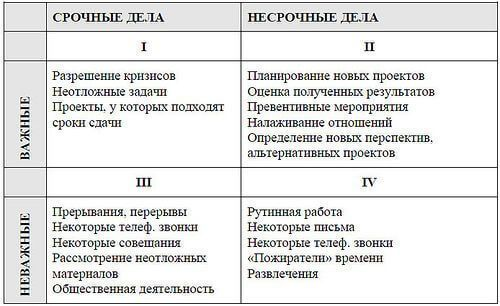
\includegraphics[scale=0.85]{images/eizinhower.jpg}  
  \caption{ Матрица Эйзенхауэра. }
  \label{fig:domain:eizenhower}
\end{figure}

\subsubsection{Квадрант A: важные и срочные дела }


При идеальном планировании этот квадрант матрицы должен оставаться пустым, т.к. появление важных и срочных дел является показателем неорганизованности и допущения завала. Эта часть графика заполняется у многих людей из-за присущей им лени и неправильной расстановки приоритетов. Естественно, временами подобные дела могут появляться у каждого человека, но если это происходит ежедневно, то самое время обратить внимание на самодисциплину.

Итак, появления дел в квадранте A следует избегать. А для этого необходимо лишь вовремя выполнять пункты остальных квадрантов. Но если в первый квадрант что-то всё же и стоит вписывать, то это:

    Дела, невыполнение которых отрицательно сказывается на достижении поставленных целей
    Дела, невыполнение которых может стать причиной затруднений и неприятностей
    Дела, которые имеют отношение к здоровью

Важно также помнить о том, что существует такое понятие как «делегирование». Это означает, что при появлении в вашем квадранте A дел, которые можно кому-либо перепоручить, этой возможностью следует непременно воспользоваться для того чтобы как можно быстрее урегулировать другие важные и срочные дела.

\subsubsection{Квадрант B: важные, но не срочные дела }


Второй квадрант заслуживает наибольшего внимания, т.к. дела, находящиеся именно в нём, являются наиболее приоритетными и перспективными, и именно из них должны состоять повседневные задачи любого человека. Замечено, что люди, которые занимаются преимущественно делами этого квадранта, достигают в жизни наибольших успехов, продвигаются по службе, зарабатывают больше денег, имеют достаточно свободного времени и живут счастливой и насыщенной жизнью.

Обратите внимание также и на то, что отсутствие срочности позволяет подходить к решению любых задач более обдуманно и конструктивно, а это в свою очередь позволяет человеку раскрывать свой потенциал в полной мере, самостоятельно продумывать все нюансы своей деятельности и управлять временными рамками своих дел. Но здесь, помимо всего прочего, нужно помнить, что дела, находящиеся в квадранте B, если их не выполнять своевременно, могут с лёгкостью попасть в квадрант A, став ещё более важными и требующими скорейшего выполнения.

Опытные специалисты по тайм-менеджменту рекомендуют включать в квадрант B все текущие дела, связанные с основной деятельностью, планирование и анализ работы, учебные и спортивные занятия, соблюдение оптимального графика и режима питания. Т.е. всё то, из чего состоит наша обычная повседневность.

\subsubsection{Квадрант C: срочные, но не важные дела }


Дела, которые находятся в этом квадранте, по большей части являются отвлекающими и нисколько не приближающими человека к намеченным результатам. Нередко они просто мешают сосредоточению на действительно важных задачах и снижают эффективность. Главное при работе с матрицей – не перепутать срочные дела из квадранта C со срочными делами из квадранта A. Иначе образуется неразбериха и то, что должно быть выполнено в первую очередь, остаётся на втором плане. Всегда помните о своих целях и учитесь отличать важное от второстепенного.

К делам квадранта C можно отнести, к примеру, навязанные кем-либо со стороны встречи или переговоры, празднования дней рождения не очень близких людей, внезапно возникшие хлопоты по дому, устранение не жизненно важных, но требующих внимания отвлекающих факторов (разбилась ваза, сломалась микроволновая печь, перегорела лампочка и т.п.), а также другие всевозможные дела, которые не продвигают вас вперёд, а только тормозят.

\subsubsection{Квадрант D: не срочные и не важные дела }


Задачи, относящиеся к последнему квадранту, не приносят совсем никакой пользы. Во многих случаях полезно не только заниматься ими в последнюю очередь, но и не заниматься ими вообще. Хотя знать о них непременно нужно, т.к. именно они являются «пожирателями времени».

Интересна и ещё одна особенность дел из данной группы: они являются очень привлекательными для многих людей – эти дела просты в выполнении и доставляют удовольствие, позволяют расслабиться и приятно провести время. Поэтому и противостоять соблазну ими позаниматься бывает довольно проблематично. Но делать это непременно нужно.

В квадрант D можно записать такие дела как разговоры по телефону с друзьями о чём-то несущественном, ненужная переписка или времяпрепровождение в соцсетях, просмотр сериалов и различных «отупляющих» телепередач, компьютерные игры и т.п. Конечно, отдыхать и как-то развлекать себя периодически должен каждый человек, но для этого существуют и более интересные и развивающие способы: чтение хороших книг, интеллектуальные игры, посещение спортзалов и бассейнов, поездки на природу и т.п. Если же полностью избавить себя от занятия делами из квадранта D не удаётся или не хочется, то нужно отложить их выполнение хотя бы до того момента, когда дела из квадрантов B и C будут выполнены, а время, которое 